\subsection{UML-Диаграммы}

UML (англ. Unified Modeling Language – унифицированный язык моделирования) – язык графического описания для объектного моделирования в области разработки программного обеспечения, моделирования бизнес-процессов, системного проектирования и отображения организационных структур \cite{uml}. 

UML является языком широкого профиля, это – открытый стандарт, использующий графические обозначения для создания абстрактной модели системы, называемой UML-моделью. UML был создан для определения, визуализации, проектирования и документирования, в основном, программных систем. UML не является языком программирования, но на основании UML-моделей возможная генерация кода \cite{uml}. 

Использование UML позволяет также разработчикам программного обеспечения достигнуть соглашения в графических обозначениях для представления общих понятий, таких как класс, компонент, обобщение, агрегация и поведение, и больше сконцентрироваться на проектировании и архитектуре. 

Далее рассмотрим следующие виды диаграмм:
\begin{itemize}
	\item диаграмма прецедентов (диаграмма поведения);
	\item диаграмма компонентов (структурная диаграмма);
	\item диаграмма последовательности (диаграмма взаимодействия);
	\item диаграмма деятельности (диаграмма поведения).
\end{itemize}

\subsubsection{Диаграммы прецедентов}

Диаграмма прецедентов (диаграмма вариантов использования) – диаграмма, на которой отражены отношения, существующие между актёрами и вариантами использования. Актёрами называют некоторые роли, определенные для разрабатываемого проекта, которые пользователь принимает по отношению к системе. Вариантами использования называют возможные действия, которые пользователь может совершить в контексте роли, которую он представляет.

Основная задача – представлять собой единое средство, дающее возможность заказчику, конечному пользователю и разработчику совместно обсуждать функциональность и поведение системы.

Для отражения модели прецедентов на диаграмме используются:
\begin{enumerate}
	\item[1] Рамки системы (англ. system boundary) – прямоугольник с названием в верхней части и эллипсами (прецедентами) внутри. Часто может быть опущен без потери полезной информации.
	\item[2] Актер (англ. actor) – стилизованный человечек, обозначающий набор ролей пользователя (понимается в широком смысле: человек, внешняя сущность, класс, другая система), взаимодействующего с некоторой сущностью (системой, подсистемой, классом). Актёры не могут быть связаны друг с другом (за исключением отношений обобщения/наследования).
	\item[3] Прецедент – эллипс с надписью, обозначающий выполняемые системой действия (могут включать возможные варианты), приводящие к наблюдаемым актёрами результатам. Надпись может быть именем или описанием (с точки зрения актёров) того, «что» делает система (а не «как»). Имя прецедента связано с непрерываемым (атомарным) сценарием – конкретной последовательностью действий, иллюстрирующей поведение. В ходе сценария актёры обмениваются с системой сообщениями. Сценарий может быть приведён на диаграмме прецедентов в виде UML-комментария. С одним прецедентом может быть связано несколько различных сценариев.
\end{enumerate}

Для проектируемого проекта, диаграмма прецедентов будет иметь следующий вид (рисунок).

\begin{figure}[h!]
	\centering
	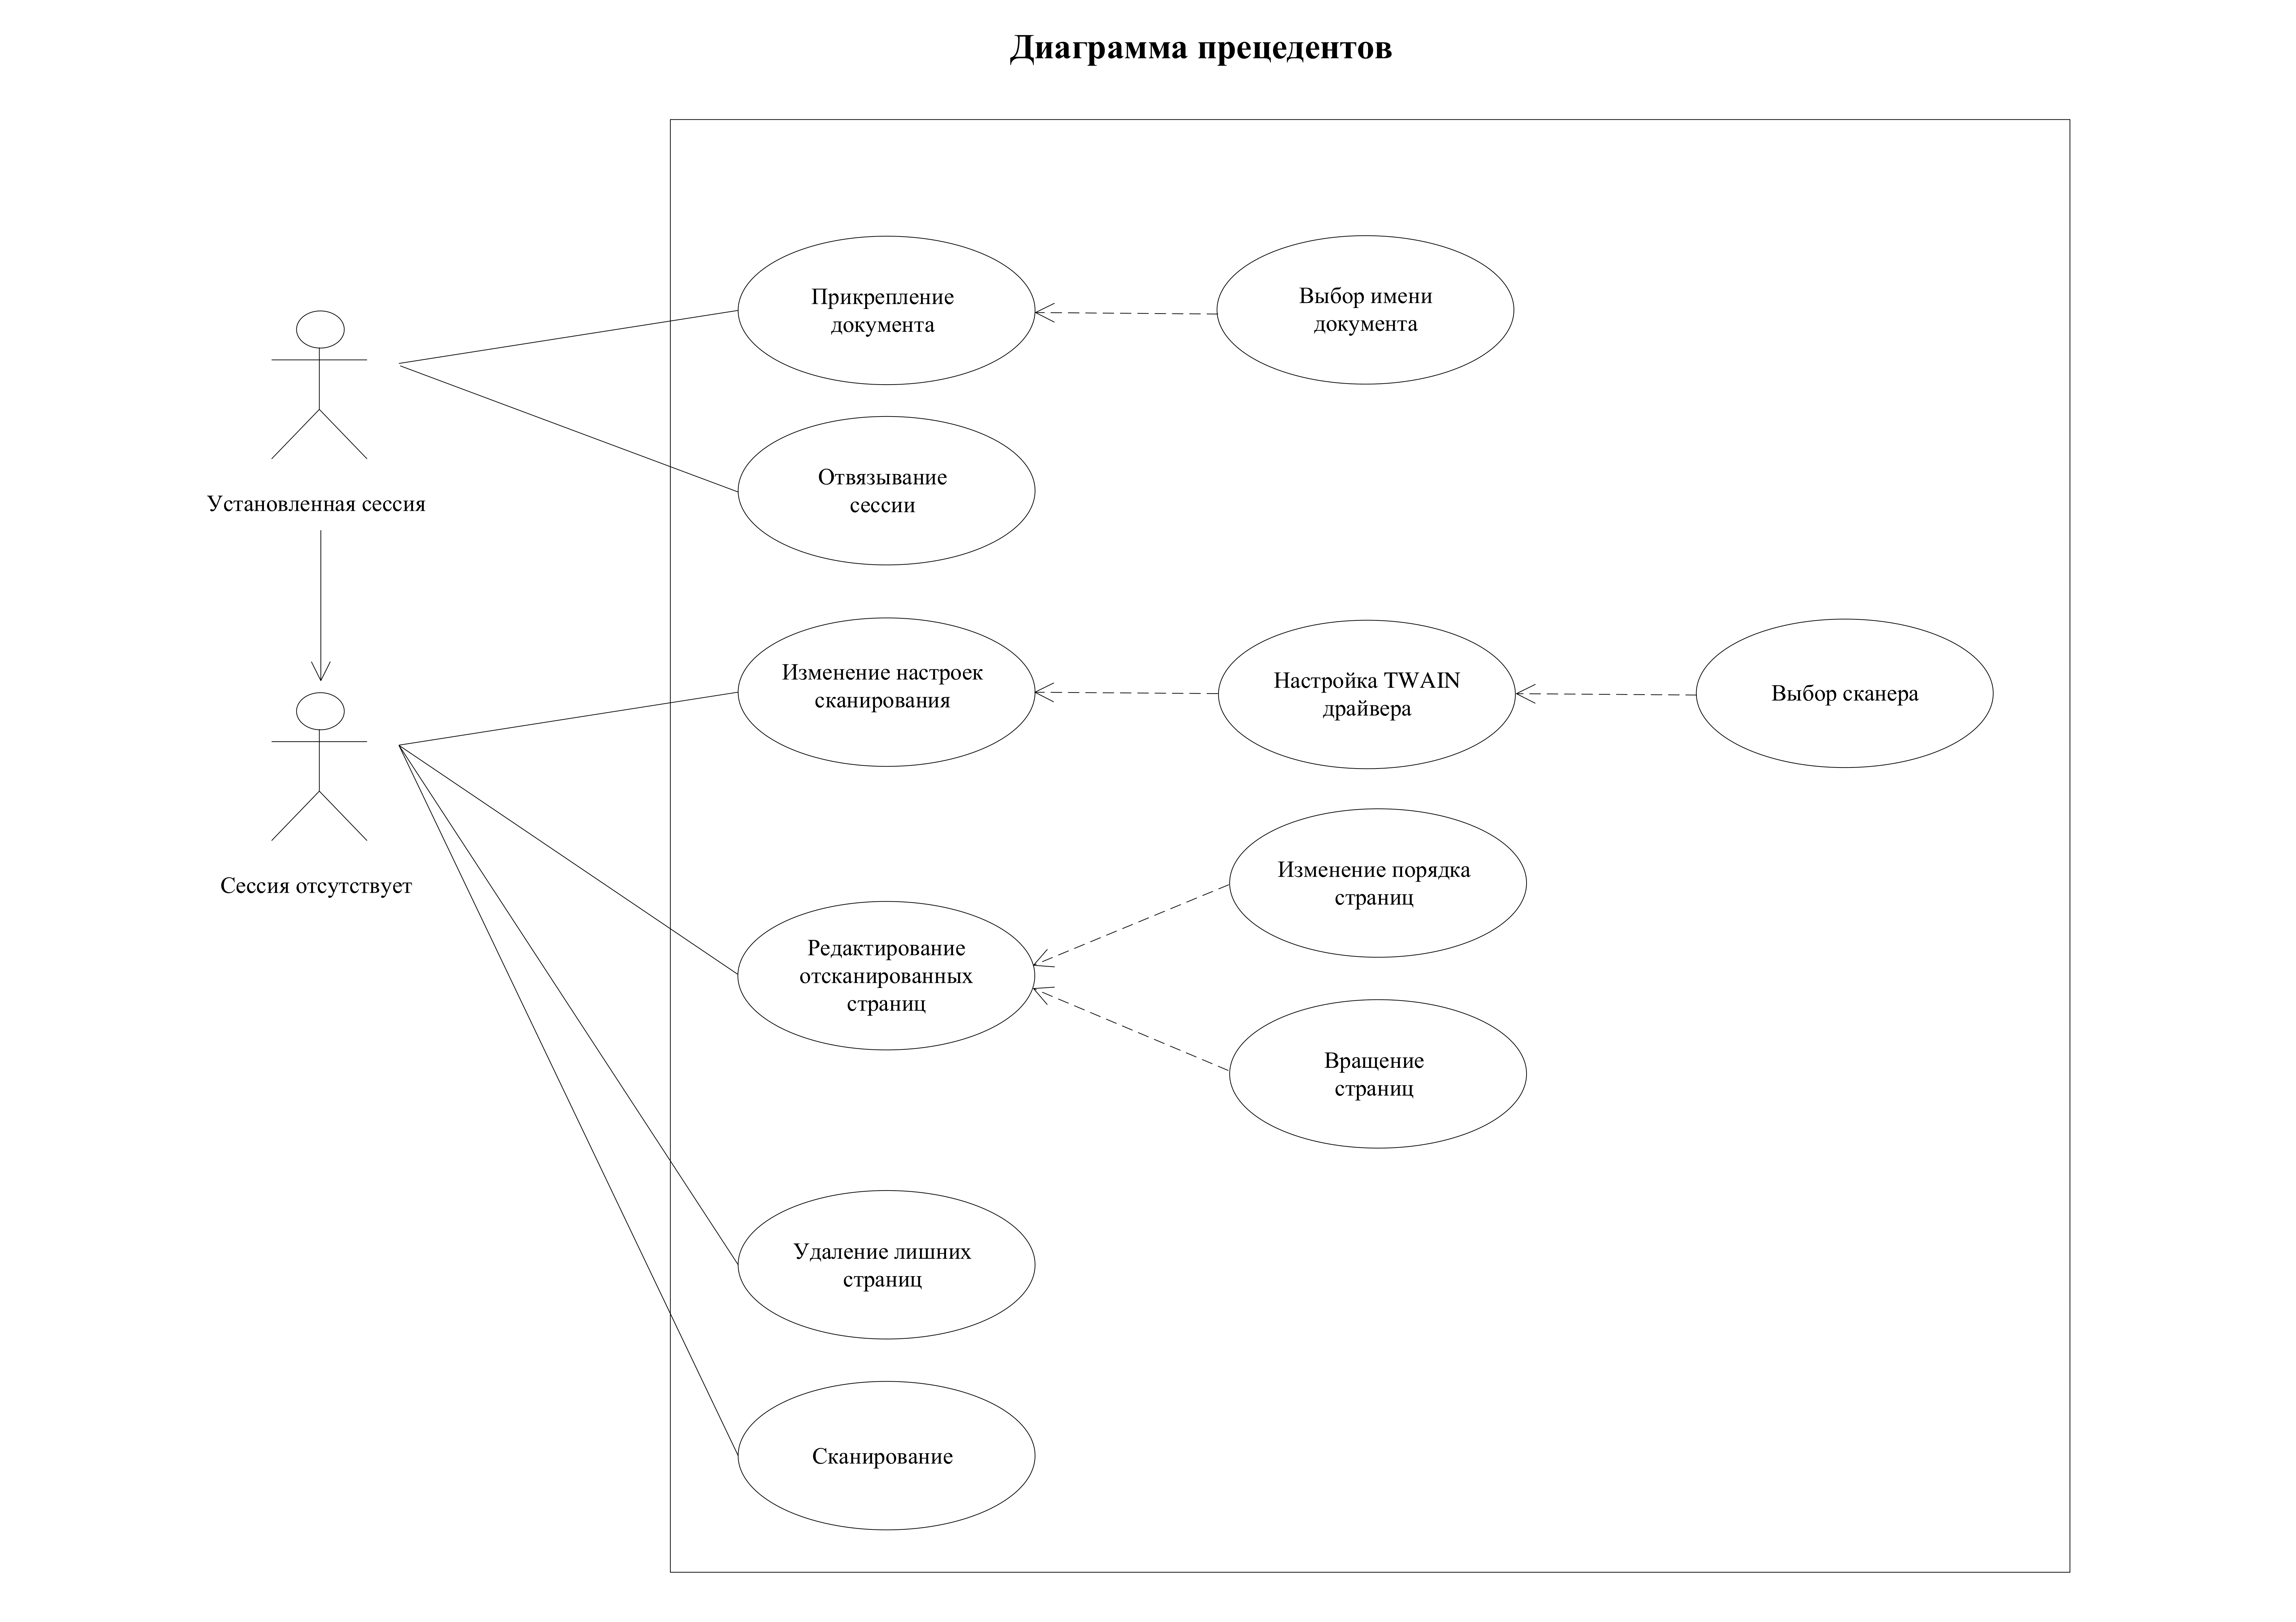
\includegraphics[scale=0.078]{pl2_precendent.png}
	\caption{Диаграмма прецендентов}
\end{figure}

В рамках проектируемого проекта, подразумевается две роли (т.е. два актера):
\begin{enumerate}
	\item[1] Пользователь, который уже привязал сессию СЭД к приложению. Такой пользователь может прикреплять документы на основе привязанной сессии. Так же такой актер может производить все остальные действия, доступные пользователю без сессии.
	\item[2] Пользователь, который не прикрепил сессию. У такого актера есть возможность сканировать документы, редактировать отсканированные документы, но нет права прикреплять документы. Для получения этого права нужно зайти в веб версию СЭД и запустить оттуда сканирование.
\end{enumerate}

\subsubsection{Диаграммы последовательностей}

При программировании некоторых функций проекта, бывает полезно иметь план взаимодействия объектов, это позволяет следовать каждому пункту, заранее разработанного, плана, не задумываясь как все должно работать вместе, что позволяет избежать многих ошибок и, как следствие, спасает разработчика от постоянной переработки логики. Для составления таких планов взаимодействия существуют диаграммы взаимодействия.

Диаграмма взаимодействия – диаграмма, которая описывает взаимодействие определённых объектов в различных ситуациях и условиях их поведения. В языке UML существует несколько типов диаграмм взаимодействия, самым популярным из них являются диаграммы последовательностей.

Диаграмма последовательности (sequence diagram) – диаграмма, которая на временной оси показывает жизненный цикл какого-либо определённого объекта (создание, уничтожения или деятельность некоторой сущности) для некого набора объектов.

Основными элементами диаграммы последовательности являются:
\begin{enumerate}
	\item[1] Объекты. На диаграмме изображаются как прямоугольниками с названиями объектов.
	\item[2] Линии жизни. На диаграмме изображаются пунктирными, вертикальными линиями, отражают течение времени.
	\item[3] Прямоугольники, которые отражают деятельность объекта или исполнение им определенной функции. На диаграмме размещаются на пунктирной линии жизни.
	\item[4] Стрелки, показывающие обмен сигналами или сообщениями между объектами.
\end{enumerate}

Одна из основных возможностей пользователей приложения – прикрепление отсканированных документов. Этот процесс взаимодействует с браузерным приложением СЭД, сканером а так же сервером, на который будут отправляться отсканированные документы.

Рассмотрим диаграмму последовательности для процесса прикрепления файла (рисунок 5.6).

\begin{figure}[h!]
	\centering
	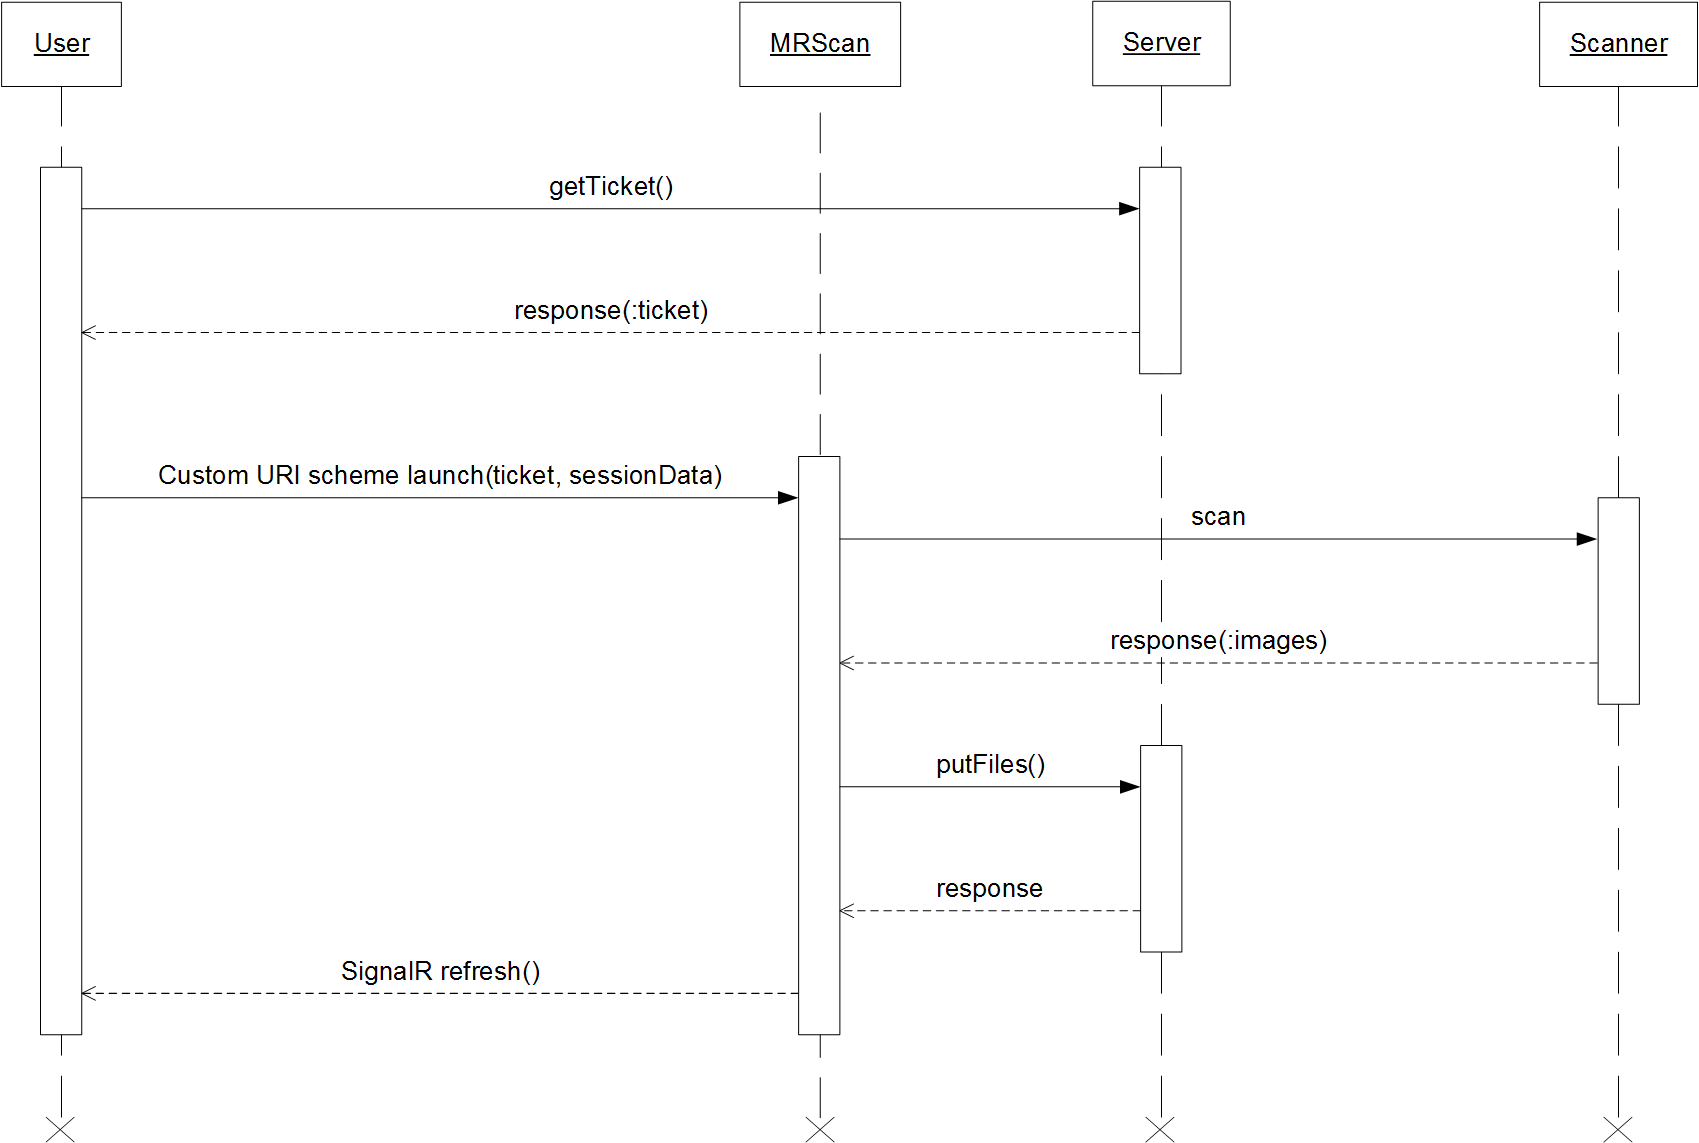
\includegraphics[scale=0.38]{pd3_sequence_general_withoutHeader.png}
	\caption{Диаграмма основной последовательности прикрепления файлов}
\end{figure}

Запуск процесса инициируется пользователем по нажатию на кнопку «Сканировать» в веб-приложении. По нажатию на данную кнопку, требуется запросить создание тикета, который будет использован в дальнейшем для прикрепления файлов. Тикет создается на серверной части. Сервер возвращает идентификатор тикета и время его создания. Далее через Custom URI запускается главное приложение (MRScan), так же через Custom URI передается вся необходимая информация. После запуска приложения, пользователь может начинать сканирование документов. Для этого действия требуется нажать на кнопку «Сканировать», на этот раз в MRScan. Нажатие на кнопку запускает сканирование, отсканированные странички начнут добавляться в список по мере сканирования. Когда сканирование завершится у пользователя есть возможность внести изменения в порядок следования страниц, а так же повернуть страницы, которые могли быть вставлены неверной стороной. Если некоторые страницы были ошибочно переданы сканеру, либо сканирование было осуществлено некачественно, есть возможность удалить ненужные страницы. Когда пользователь определился с контентом будущего докумкнта, он нажимает кнопку «Прикрепить», это запускает функцию putFiles(), в которой на основе ранее полученных данных через Custom URI, создается тикет и на основе тикета, вызывается метод WCF сервиса, который отправляет прикрепляемый файл на сервер окуда он попадает в базу данных. После того как файл успешно прикрепился, MRScan отправляет через SignalR сообщение веб-приложению, которое обновляет страничку и сразу отображает прикрепленный файл. 

\begin{figure}[h!]
	\centering
	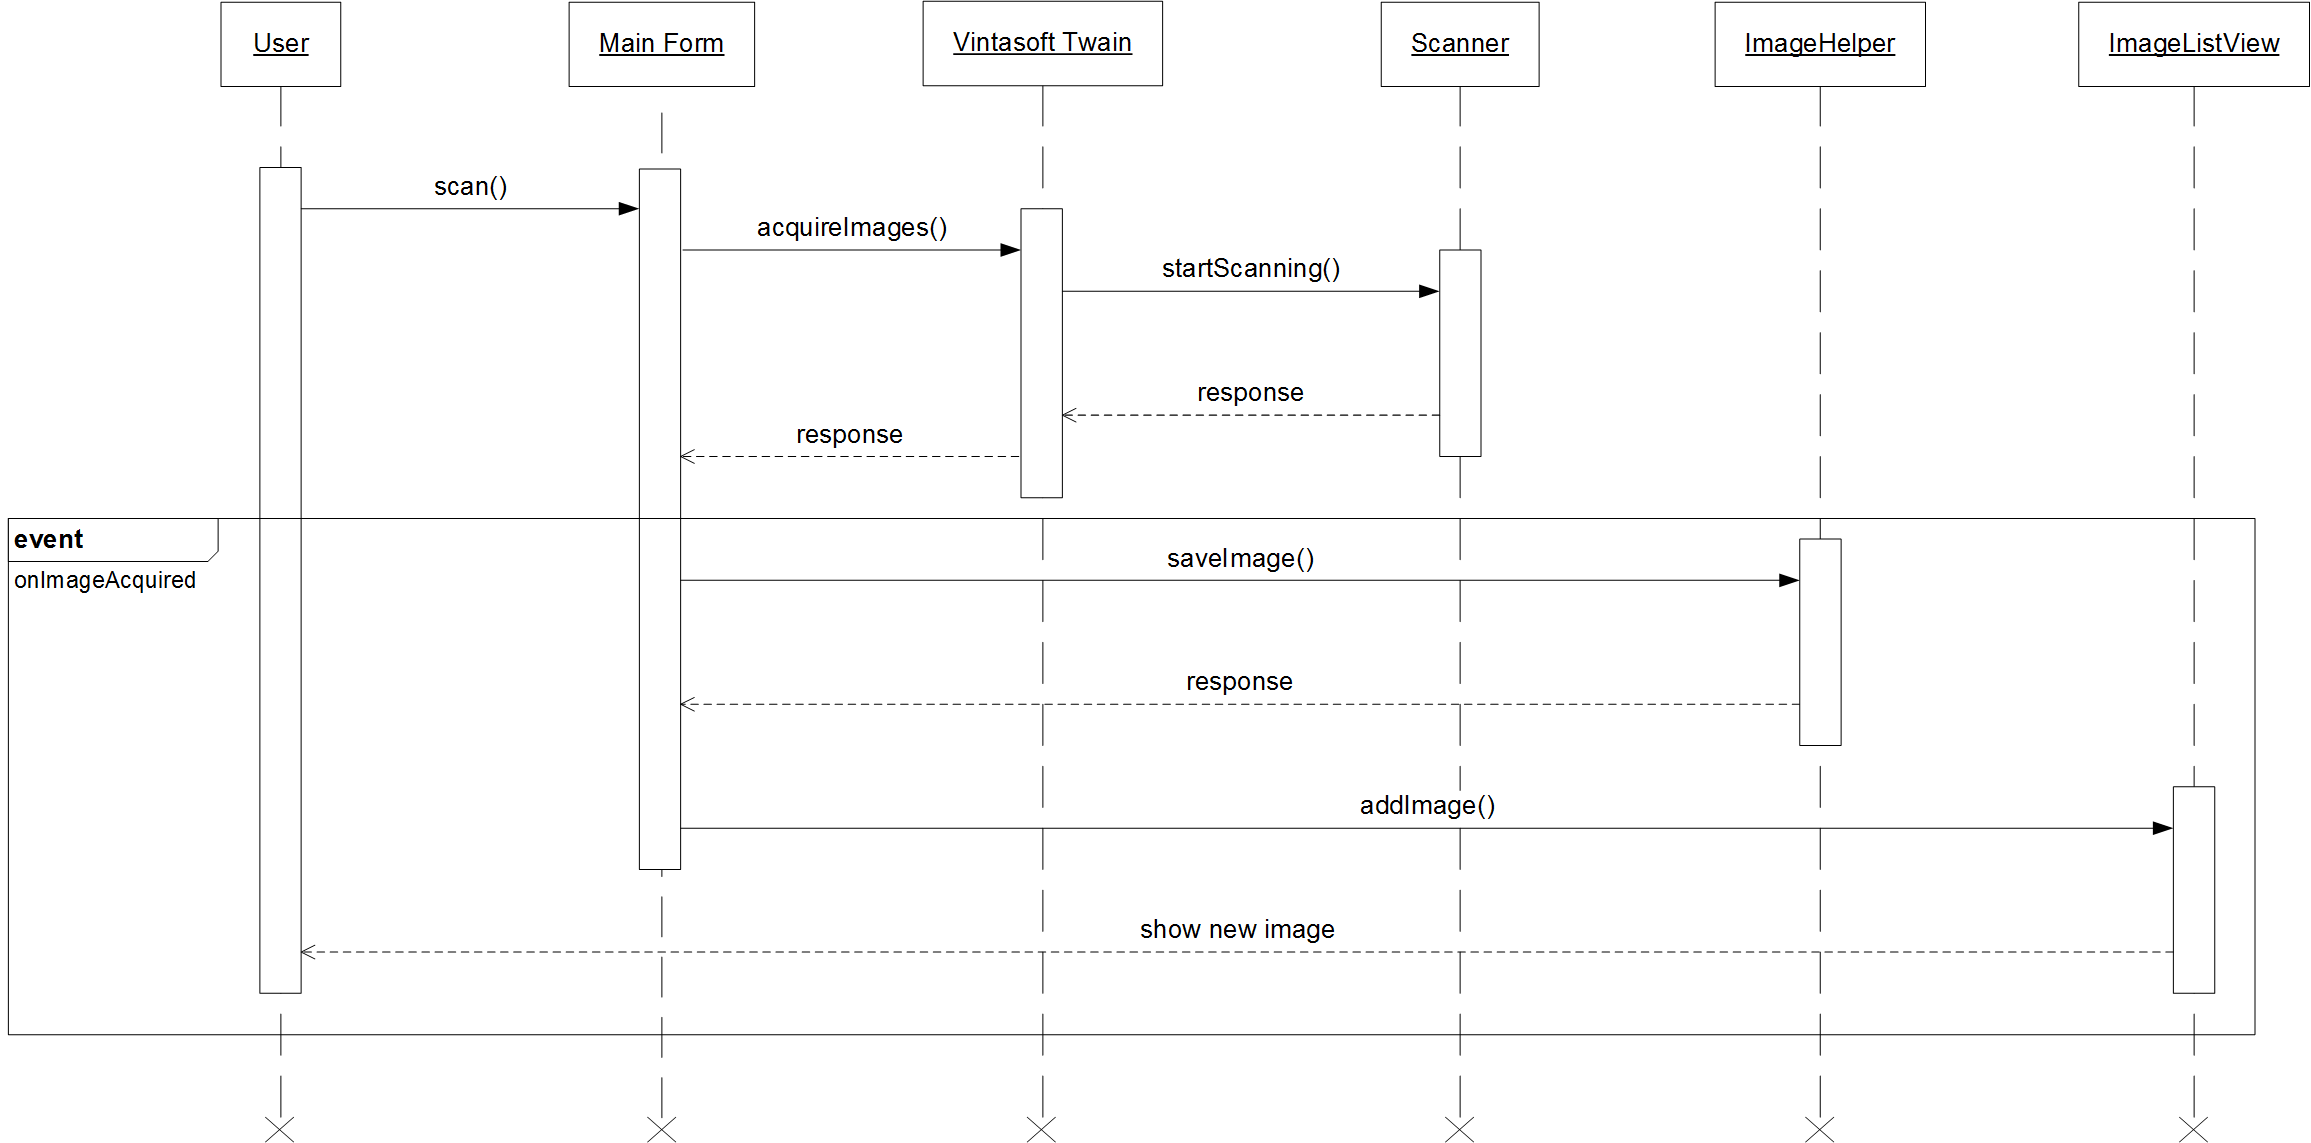
\includegraphics[scale=0.3]{pd4_sequence_withoutHeader.png}
	\caption{Диаграмма последовательности сканирования}
\end{figure}